% !TeX root = ../../master_thesis.tex

\section{Historical aspect of Artificial Intelligence}

\subsection{Decision Support Systems} 

One of the earliest versions of computer intelligence implementations were Decision Support Systems.
Decision Support Systems are interactive, computer-based systems that aid users in judgment and choice activities.
They provide data storage and retrieval, but enhance the traditional information access and retrieval functions with support for model building and model-based reasoning.
They support framing, modeling, and problem-solving.
Decision support systems are typically used for strategic and tactical decisions faced by upper-level management—decisions with a reasonably low frequency and high potential consequences—in which the time taken for thinking through and modeling the problem pays off generously in the long run.
\cite{decision_support_systems_article}

There are three fundamental components of Decision Support Systems: database management system — DBMS, model-base management system — MBMS, and dialog generation and management system — DGMS.
\cite{decision_support_systems_engineering}

A DBMS serves as a data bank for the Decision Support System. 
It stores large quantities of data that are relevant to the class of problems for which the DSS has been designed and provides logical data structures (as opposed to the physical data structures) with which the users interact. 
A DBMS separates the users from the physical aspects of the database structure and processing. 
It should also be capable of informing the user of the types of data that are available and how to gain access to them.

The role of MBMS is analogous to that of a DBMS. 
Its primary function is providing independence between specific models that are used in a DSS from the applications that use them. 
The purpose of an MBMS is to transform data from the DBMS into information that is useful in decision-making. 
Because many problems that the user of a DSS will cope with may be unstructured, the MBMS should also be capable of assisting the user in model building.

The main product of an interaction with a DSS is insight. 
Because their users are often managers who are not computer trained, DSSs need to be equipped with intuitive and easy-to-use interfaces. 
These interfaces aid in model building, but also in interaction with the model, such as gaining insight and recommendations from it.
The primary responsibility of a DGMS is to enhance the ability of the system user to use and benefit from the DSS. 
In the remainder of this entry, we use the broader term user interface rather than DGMS.

First attempts to create and use AI in Decision Support Systems by banks had started in 60s-70s.
Back then, it sounded as something definitely impossible.
Unfortunately, existing state of science wasn't able to satisfy banks' needs and first experience of AI implementation was done only a few decades later.
The pioneer of implementation of Artificial Intelligence System was Citibank.
Specialists of this company made an attempt to implement an automatic Decision Support System that could be as effective, as human experts and more cost-effective.
Generally, Citibank had gotten positive summary.
\cite{decision_support_systems_book}

As a result, leading banks in the United States tried to apply and implement AI as their business solution.
However, due to, comparing with present, low level of development of information technologies, banks found application of AI economically unjustified.
Banks did not invest in continuing researches and for the couple of decades forgot about AI.



\subsection{Contemporary history}

Historically, banks became large financial entities with lots of regulations over them.
This requires from banks humongous levels of responsibility and accountability.
Consequently, banks are known as owners of enormous amount of data, which may be required by regulators, as well as by clients.
Nevertheless, banks are highly interested in using those amount of data for business purposes.
However, both collecting, maintaining, processing input data and using output results is not a simple set of operation.
Having mainly numerical data in digital form, this set of operation requires significant work in terms of Mathematics, Statistics and Computer Science.
This becomes extremely complicated due to previously mentioned gigantic amounts of data, which can easily overpass 1 Terabyte of data a day.

Therefore, that was not a surprise, that Commercial Banking was always keeping its eye on evolution of related technologies.

Even though, banks were using synergy of Mathematics, Statistics and Computer Science since 1950s with varied success, the latest big forward jump was in early 2010s. 

By then, ability to accumulate and process large amounts of data became essential for multiple industries, not only the one, that historically accumulate data. 
\cite{forbes_big_data_history}
Those large amounts of data are usually referred to as Big Data.
Big Data are information assets characterized by such a High Volume, Velocity and Variety to require specific Technology and Analytical Methods for its transformation into Value.
\cite{what_is_big_data}

Since early 2010s, consumer banks started adoption of fast growing Big Data technologies. 
Banks, historical owners of enormous amounts of data, were extremely interested in Big Data solutions and specialists. 
Even though Big Data solves problems regarding collection, maintenance and preprocessing of data, additional tools are required for general processing, data usage and application.
Those tools are provided by Machine Learning.

Most recent advances in AI have been achieved by applying machine learning to very large data sets. 
Machine Learning algorithms detect patterns and learn how to make predictions and recommendations by processing data and experiences, rather than by receiving explicit programming instruction. 
The algorithms also adapt in response to new data and experiences to improve efficacy over time. 
\cite{executive_guide_to_ai}

Obviously, even after decades of research and development those technologies had been still considered as a bit risky.
Therefore, banks had decided to start with something, that would allow reducing costs or optimizing non-operational activity.

On June 2016, agency Reuters issued an article\cite{reuters_ai_hiring}, in which it mentioned that banks of Wall Street in order to try to decrease costs were looking into software development, so it could help to optimize and to speed up the process of searching suitable employees.
For highest performance and due to unpredictable results, banks had bet on Artificial Intelligence.
AI technologies would allow discovering and identify in applicants such qualities, that would be proficient for employer, including ability to works in a team, with a big purpose, willpower, and other soft skills, that,  probably, wouldn't be mentioned in CV or could be found out during interview process.
Hires of bad candidates can cost a lot for a company and lead to large financial expenses and influences negatively for company's business possibilities.
According to experts of Capital One Financial, those losses in average are three salaries of a person, who could fit perfectly for this job.
In such cases self-developing algorithms may allow its clients to get rid of such human errors, as screening out strong candidates, that may look weak at once.
The possibility of implantation of AI to a common process is being under consideration by such financial giants as Goldman Sachs Group, Morgan Stanley, Citigroup and UBS Group.
UBS Group had started using algorithms, that allows to analyze CVs and to find tough candidates as well.
Goldman Sachs Group had used its own software to find specific qualities in CVs, for example, teamwork, honesty and judiciousness.
Furthermore, it uses personality tests for better understanding of qualities of successful bankers and traders.
Some banks used third-party solutions.
For example, Citigroup in June 2016 started testing technology, developed by third-party, to dropout candidates.
Software had been tested on a small group of employees, who had been working in corporate and investment departments.
The application determines, so called, “corporate imprint” — certain set of qualities of existing employees,
which should lead to high corporate performance — and evaluates qualities of candidate based on 
small video, on which job seekers are talking about their strengths and aspirations in career.
That system takes into account not only specific features of job seeker's speech, but also one's skill to present his speech, including body language and rate of speech.
Previously, technologies allowed and helped to find out the best CV, while nowadays it allows understanding people, that apply for a job.
Such solutions give a possibility to drastically remove expenses for unsuccessful hiring and improve the situation on labor market.
In general, Artificial Intelligence allow selecting candidates, that will be able to execute needed work, as it can create templates, based on analysis of big volumes of data.

It may seem, that the changes affected only European and US banks, but AI became a main trend on Asian markets as well.
In Japan, by the end of 2017, it became known about the plans of leading Japanese banks to automate about 30 thousand workplaces until 2027.
Bank boards reached a conclusion, that automatization is inevitable, due to the fact, that traditional methods of making business would not help in increasing incomes.
It would allow minimizing costs of labor capital and direct it to fields, where human workforce would be more valuable.

Those banks assumed, that existing, traditional, business model didn't allow increasing financial gains.
Leading Japanese banks and financial companies, Mizuho Financial Group, Sumitomo Mitsui Financial Group and Bank of Tokyo-Mitsubishi UFJ, informed about readiness to automate more than 30 thousand working places. 
\cite{nikkei_30000_jobs}

According to Nikkei, Mizuho Financial Group are going to replace around 8 thousand employees with computers and increase that number up to 19 thousand.
Sumitomo Mitsui Financial Group started moving towards large-scale automation.
Based on their plans, they were expecting to automate around 4 thousand workplaces by the end of 2020.
Group considered consolidating various clerical work to minimize amount of staff with duplicating duties.
Moreover, around 100 generic routine work tasks would be done by new robotized processing system, that previously had been used by Mizuho Financial Group only for data inputting on opening new investment accounts on its website.
What is even more important, large-scale digitalization did not imply layoffs.
For example, Sumitomo Mitsui Financial Group started its transformation by transferring around 200 back office employees to customer service departments.
Besides, Mizuho Financial Group intends to increase the number of financial technology specialists.
Mitsubishi UFJ keeps up with competitors and plans to automate 9500 jobs up to FY 2023. \cite{mufj_digital_strategy}


Nowadays, the largest market, that uses AI as a solution in the banking sector, remains North America.

In June 2018 Bank of America announced start of research process of using of Machine Learning or currency strategies analysis.
Announced reason for the research was the unstable political situation in Italy — experts feared that it would have a negative influence both on Euro and other European currencies, and this threatens to create new financial crisis.
In the first research Bank of America algorithms of Machine Learning were evaluated by performance of working with fundamental and review data, that involve, for example, governmental costs and expectation of consumer.
The main task of an AI is to create a forecast of relationships of euro and dollar pair.
Due to the nature of the foreign exchange market, it’s rather difficult to forecast using only known situations, and as a result Machine Learning may allow identifying unexpected existing unknown patterns.
\cite{bank_of_america_ai}

As other banks, Wells Fargo \& Company applied Artificial Intelligence in Front Office for customer experience and in Middle Office, for anti-money laundering.
Nevertheless, Wells Fargo \& Company declared that it additionally adheres to a fundamental economic approaches for analysis of foreign exchange markets, as it trusts its experience in this field.
\cite{wells_fargo_ai}

As an example, commercial bank Morgan Stanley hired Michael Kearns, professor of Applied Informatics in Pennsylania University, who had been working in a hedge fund previously, in order to expand the use of AI, while research team of Deutsche Bank had started using Machine Learning for its data analysis.

On the other side, some players did not want to take a risk.
JP Morgan Financial Holdings Research Group had been studying applications for Machine Learning for a long time, but had not decided to use it until year 2021.
Only in first half of 2021 JP Morgan hired 50 artificial intelligence experts and plans to hire at least 160 more professionals.
\cite{jp_morgan_ai}

The fact, that banks are more actively using Artificial Intelligence in applied work was confirmed by Deloitte.
Based on Deloitte research, 
29\% of financial companies, working in different countries, automate most of monotonic routine processes,
25\% respondents use such technologies for risk management,
21\% — for generating risk reports, 
20\% — for regulatory reporting.
\cite{deloitte_thriving_in_ai_era}


The Financial Times made special survey for 30 largest banks, which confirmed a close interest and an understanding of resulting impact 
of swift implementation of modern operation technologies.
Among 18 banks, 17 do already use Artificial Intelligence in clients communication, as it is on this site that they see the most obvious benefits.
8 banks use AI in all structural divisions in any form.
5 expecting in future to have special divisions, which will focus on AI.
8 involved in joint development with specialized companies. 
Moreover, 4 of those even invested into companies, which are exploring AI.
\cite{ai_reality_hype}


Big data and data analysis are still prioritized for banks, as 40\% of respondents use it in everyday data processing.
Around 25\% of respondents declared usage of Machine Learning and 19\% of Cognitive Analytics, including Natural Language Processing, in order to decrease costs and increase operational accuracy, while 24\% of asked banks use it for Business Intelligence.



All over the world, in general in 2018 banks income due to application of Artificial Intelligence was around \$41.1 billion. 
It is important to note, that this amount contains both direct income from implementation of AI technologies, but also
an amount of decreased costs and benefits due to increased work effectiveness of various financial structures, comparing with work effectiveness using same old processes and infrastructures.
And according to market forecasting this income will only grow.
\cite{ihs_markit}

\begin{figure}
    \centering
    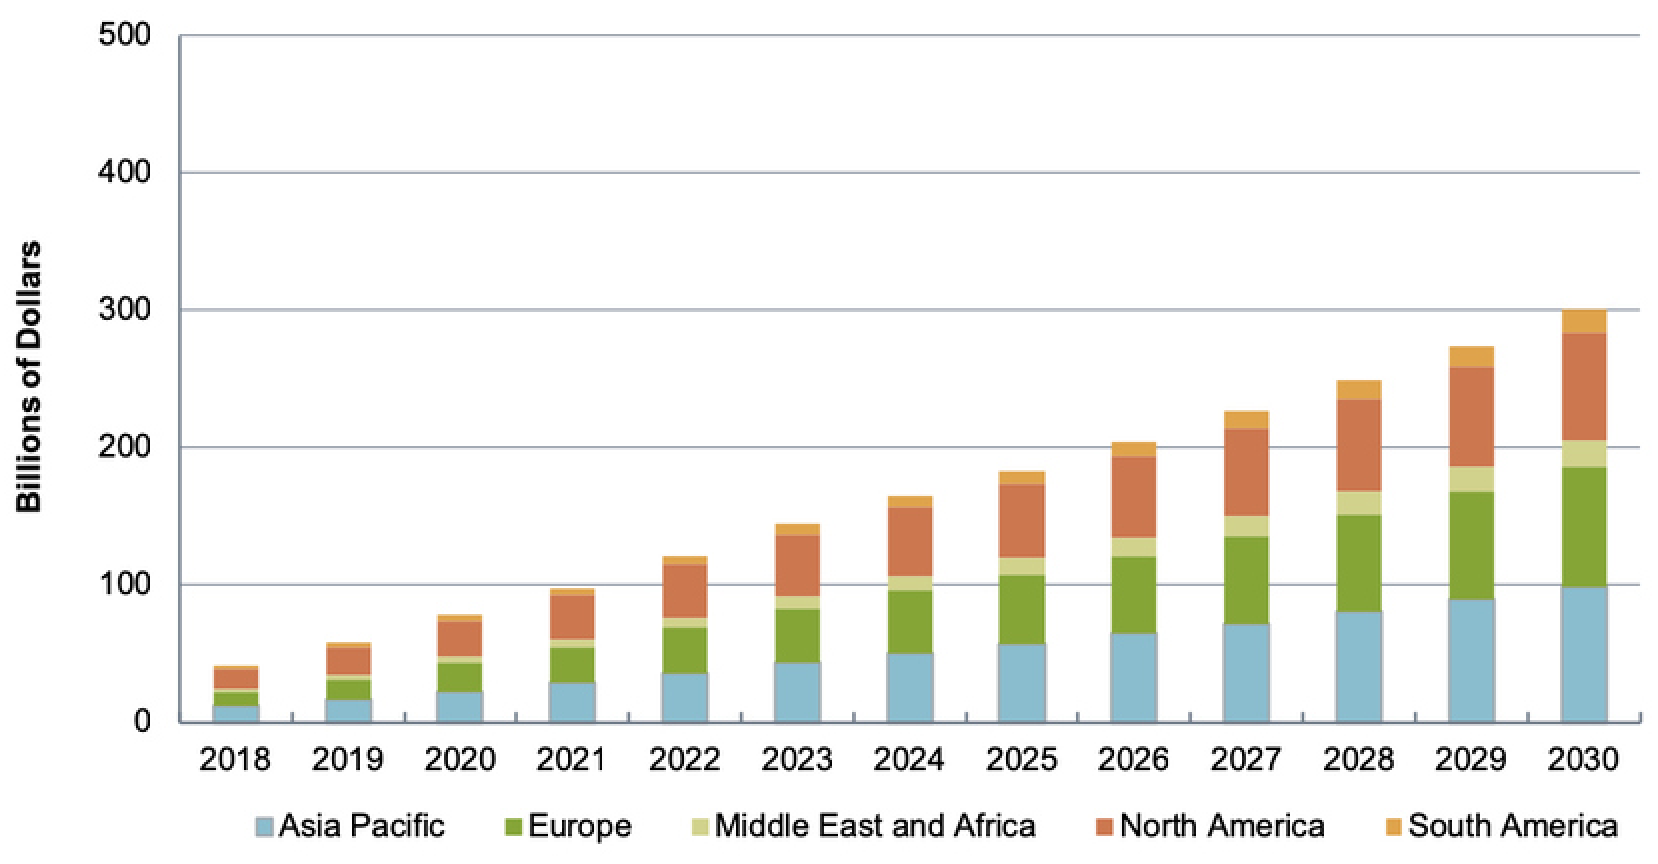
\includegraphics[width=0.8\textwidth,height=\textheight,keepaspectratio]{images/Banking_AI_Business_Value.png}
    \caption{The business value for the world market for AI in banking by region}
    \medskip
    \footnotesize\textit{Source:} "Artificial Intelligence in Banking Report", IHS Markit, 2019, p. 10.
\end{figure}

Even though, as previously mentioned, United States banks are leaders of Artificial Intelligence application, where companies earned additional \$14.7 billion in 2018 thanks to those technologies, experts expect that by 2024 the Asia-Pacific region will break out into the lead, as banks expect to earn and save, thanks to AI, around \$50.6 billion, while in 2018 those banks saved \$11.5 billion.
By 2030 it will raise up to \$98.6 billion due to demand in China (including Hong Kong), Japan, South Korea and Singapore.
\cite{ihs_markit}

According to forecasters, by 2030 banks in the whole world would be able to decrease costs by 22\% using Artificial Intelligence technologies. 
In numbers, this reduction can reach \$1 trillion.
\cite{trillion_opportunity}

According to Accenture, the amount of savings by 2035 will be nearly \$1.2 trillion.
\cite{accenture_ai_banking}

The most tangible changes will occur in units that have direct contact with customers.
By reducing amount of retail divisions, cashiers and security officers, banks cut costs by \$490 billion.
In departments responsible for data processing, analytics and reports, 
introduction of Artificial Intelligence will save up to \$350 billion in middle office and \$200 billion in back office.
In the US banking sector, more than 1.2 million of employees have already encountered AI, even thought they may not be aware of it.


Nevertheless, AI technologies should change structure of financial industry, making bank sector more humane and intelligent.


The profit for the bank is obvious, as it will result in significant cost reduce.
However, forecasts about employment in front banking are much less optimistic.
Recent study of Autonomous Research have shown, that AI can lead to 1.3 million employees losing their jobs in the United States and 500 thousand employees in Great Britain.

Former CEO of Citigroup, Vikram Pandit, who is considered as FinTech evangelist, assume that 30\% of bank employees can be replaced by Artificial Intelligence in near future. 
The threat of layoffs is real for existing bank employees.
Former CEO of Deutsche Bank told, that they intend to replace 98 thousand of workers with smart software solutions, while
Japanase Mizuho Financial Group will free 19 thousand of workplaces, third of entire stuff, by 2027. 
\cite{ai_reality_hype}


IHS Market assumes, that among bank employees, who can lose workplaces, the biggest risk is for B2C front-office workers, especially, cashiers, customer service, interviewers, clerks, financial managers, controllers and credit specialists.
\cite{ihs_markit}


Even though usage of Machine Learning for complex analysis is not an innovation, according to Vasant Dhar, Informatics Professor in New York University and founder of SCT Capital Management Hedge Fund, which has been applying AI for 20 years, foreign exchange markets are still a significant challenge for AI algorithms and modelling.
Complexity and variety of macroeconomic factors, which can have influence on inter-currency relations, crucially complicate analysis for foreign exchange markets, unlike regular stock markets that has been using AI and ML for a long time.

Main criticism of AI is based on lack of trust to results, as ML supposes Black Box analysis and finding interconnections in unpredictable ways. 
Therefore, most of the critics cannot accept prognostic findings to AI, as it processes data without building relationships
between cause and effect.

Despite rational enormous cost savings, a number of researchers are recommending to step off radicalism.
In their opinion, banks should be careful not to rely too much on new solutions.
Its effectiveness is extremely clear only in case of complementing human work, not replacing.
Therefore, introducing artificial intelligence, banks should be prepared at least to educate employees of robotized work process.
Large Dutch bank ING agrees with this position:
“We would like to use artificial intelligence in order to suggest more thoughtful decisions to our clients and to be more effective in decision-making, and not to replace workforce with AI”.
\cite{ai_reality_hype}


On this direction there is a temptation to improve the artificial intelligence, making its possibilities closer to human ones. 
Unfortunately, much still remains outside the perimeter of capabilities of modern technologies.
AI has a function of recognition, but not of cognition. 
It is wrong to assume that humans and machines can work on a same level.
It would be a long way, and it would require significant research until machines begin to at least approaching level of human performance.
Predictions regarding the timing of the creation of truly “smart” intellect are pretty vague.
\cite{ai_reality_hype}


Doubts arise not only in terms of timing.
Considerably more important are considerations of a generalized and even philosophical nature, for example, whether it is generally necessary to strive to model human thinking in its entirety.
The spheres of application of human and machine intelligence should coexist in complementarity, and not repression (or replacement)
In a number of situations, there are no simple tasks that can be solved purely algorithmically, but a human mind is needed to cope with them.
However, humanizing artificial intelligence deprives it of those strengths, for which, actually, human tries to create and swap himself with rational, algorithmic and objective source of actions and decisions.

Digital economics brings changes not only to operational bank activities, but also into relationships within community of financial institutions.

Research conducted by World Economic Forum together with Deloitte and Touché led to the conclusion that possibilities, which are being brought by Artificial Intelligence are an option only for the largest banks.
Since the main innovation concentrate on customer acquisition channels, then it is very likely to observe banking sector regroup — the dominance of large structures and the withdrawal from the market of small and medium structures.
\cite{ai_transform_disrupt}

However, researchers leave small companies a chance on survival.
Those assume that smaller companies have an option to specialize in certain directions, types of operations and specific clients.
Consequently, along with large banks, customer service in digital economics may be provided by small niche financial companies.
\cite{banking_ai_revolution}

The desire of benefit by expending of information base and Artificial Intelligence, which is the main data consumer, will lead to creation of monopolies — large alliances of financial groups.
The need of strengthening and enhancement of bank cooperation is required by increasing importance of analytical work, grow of risks of cyber-attacks and fraudulent schemes. 
The effectiveness of protection against criminals significantly increases in the conditions of sharing information about criminal patterns, sharing blacklists of companies and clients.

Nonetheless, transfer, control and usage of received data has to be settled down, including legal establishment.
Data owners, as well as clients, are interested in reliable control over data.
As a result, there is a need in obvious legal procedure of personal data transfer and its protection.
The transfer of activities to digital space creates entirely new risks and requires new methods of risk countering, which have not been worked out yet.

At the group level banks agree on a fact, that main route of development of banking is based on implementation of opportunities offered by digital economics.
Moreover, banks apply the latest achievements of computer technologies and software development, among them Artificial Intelligence, in individual areas of its work, replacing an employee with robot on routine repeating operations.
Nevertheless, banks are very careful about complete and deep technical restructuring, sending significant funds for studying the issue.
Regarding modern stage of Artificial Intelligence application and immediate prospects, I would like to cite The Financial Times:
8 years ago there was a talking robot in Santander Citi, but none of them is left in any of 13697 branches of the bank.
\cite{ai_reality_hype}

Even nowadays, banks are still focused on creating necessary conditions for AI transformations, including preparation of infrastructure, data, models and processes.
In addition to fields, that always have to be on the cutting edge, in order to gain advantage as a pioneer, 
changes are coming to more conservative spheres of financial services.
Despite the active usage of Artificial Intelligence, most banks have not had time to implement it globally yet.
According to experts, overwhelming majority of financial institutions noted usage of Machine Learning in one degree or another, but, as it had been noted by experts, only 20\% of respondents went beyond the basics of AI usage.
\cite{ai_reality_hype}

But structurally, banks were creating single open platforms, which provide general service for all domestic business customers.
Therefore, there is a need in relevant professionals, who would be able to handle and support platforms.
